\begin{figure}[t]
\centering
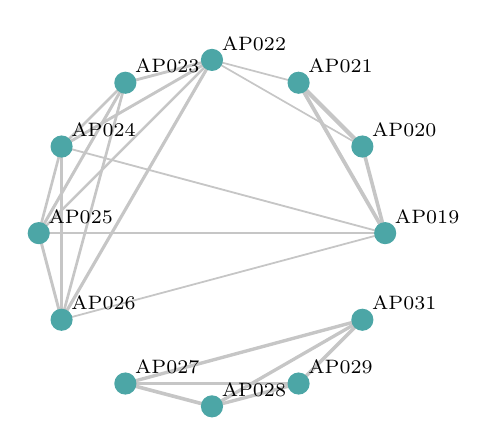
\begin{tikzpicture}[x=1cm,y=1cm, every node/.style={font=\scriptsize}]
\draw[gray!45, line width=1.50pt] (1.91,1.10) -- (1.10,1.91);
\draw[gray!45, line width=1.36pt] (2.20,0.00) -- (1.10,1.91);
\draw[gray!45, line width=1.31pt] (-1.10,-1.91) -- (-0.00,-2.20);
\draw[gray!45, line width=1.31pt] (1.10,-1.91) -- (1.91,-1.10);
\draw[gray!45, line width=1.30pt] (2.20,0.00) -- (1.91,1.10);
\draw[gray!45, line width=1.22pt] (-0.00,-2.20) -- (1.10,-1.91);
\draw[gray!45, line width=1.22pt] (-1.10,-1.91) -- (1.91,-1.10);
\draw[gray!45, line width=1.20pt] (-0.00,-2.20) -- (1.91,-1.10);
\draw[gray!45, line width=1.20pt] (-1.10,-1.91) -- (1.10,-1.91);
\draw[gray!45, line width=1.14pt] (0.00,2.20) -- (-1.91,-1.10);
\draw[gray!45, line width=1.09pt] (-1.10,1.91) -- (-2.20,0.00);
\draw[gray!45, line width=1.06pt] (-2.20,0.00) -- (-1.91,-1.10);
\draw[gray!45, line width=1.05pt] (-1.91,1.10) -- (-1.91,-1.10);
\draw[gray!45, line width=1.05pt] (0.00,2.20) -- (-1.91,1.10);
\draw[gray!45, line width=1.03pt] (0.00,2.20) -- (-1.10,1.91);
\draw[gray!45, line width=0.97pt] (-1.10,1.91) -- (-1.91,-1.10);
\draw[gray!45, line width=0.96pt] (-1.91,1.10) -- (-2.20,0.00);
\draw[gray!45, line width=0.95pt] (-1.10,1.91) -- (-1.91,1.10);
\draw[gray!45, line width=0.95pt] (0.00,2.20) -- (-2.20,0.00);
\draw[gray!45, line width=0.66pt] (2.20,0.00) -- (-1.91,1.10);
\draw[gray!45, line width=0.64pt] (2.20,0.00) -- (-1.91,-1.10);
\draw[gray!45, line width=0.62pt] (2.20,0.00) -- (-2.20,0.00);
\draw[gray!45, line width=0.62pt] (1.10,1.91) -- (0.00,2.20);
\draw[gray!45, line width=0.61pt] (1.91,1.10) -- (0.00,2.20);
\fill[teal!70] (2.20,0.00) circle (4pt);
\node[above right] at (2.20,0.00) {AP019};
\fill[teal!70] (1.91,1.10) circle (4pt);
\node[above right] at (1.91,1.10) {AP020};
\fill[teal!70] (1.10,1.91) circle (4pt);
\node[above right] at (1.10,1.91) {AP021};
\fill[teal!70] (0.00,2.20) circle (4pt);
\node[above right] at (0.00,2.20) {AP022};
\fill[teal!70] (-1.10,1.91) circle (4pt);
\node[above right] at (-1.10,1.91) {AP023};
\fill[teal!70] (-1.91,1.10) circle (4pt);
\node[above right] at (-1.91,1.10) {AP024};
\fill[teal!70] (-2.20,0.00) circle (4pt);
\node[above right] at (-2.20,0.00) {AP025};
\fill[teal!70] (-1.91,-1.10) circle (4pt);
\node[above right] at (-1.91,-1.10) {AP026};
\fill[teal!70] (-1.10,-1.91) circle (4pt);
\node[above right] at (-1.10,-1.91) {AP027};
\fill[teal!70] (-0.00,-2.20) circle (4pt);
\node[above right] at (-0.00,-2.20) {AP028};
\fill[teal!70] (1.10,-1.91) circle (4pt);
\node[above right] at (1.10,-1.91) {AP029};
\fill[teal!70] (1.91,-1.10) circle (4pt);
\node[above right] at (1.91,-1.10) {AP031};
\end{tikzpicture}
\caption{Mobility-derived AP handoff graph sample generated from the trace-compatible movement data. Edge thickness reflects relative handoff count among the strongest displayed links.}
\label{fig:generated_mobility_graph}
\end{figure}
